\subsection{Structure and mechanics}

\paragraph{}The design and operation of a CubeSat is a complex process that must be completed keeping in mind the different subsystems it has as well as their role within the satellite. Additionally, since these systems will operate in space, they have to be prepared to withstand the extreme conditions, and be certified to work properly under them. 

\paragraph{}The satellite used by Astrea must have high compatibility between all the systems to avoid potential problems during operation and has to be tested (either all the systems together or one by one) and ensure their correct functioning.


\begin{figure}[h]
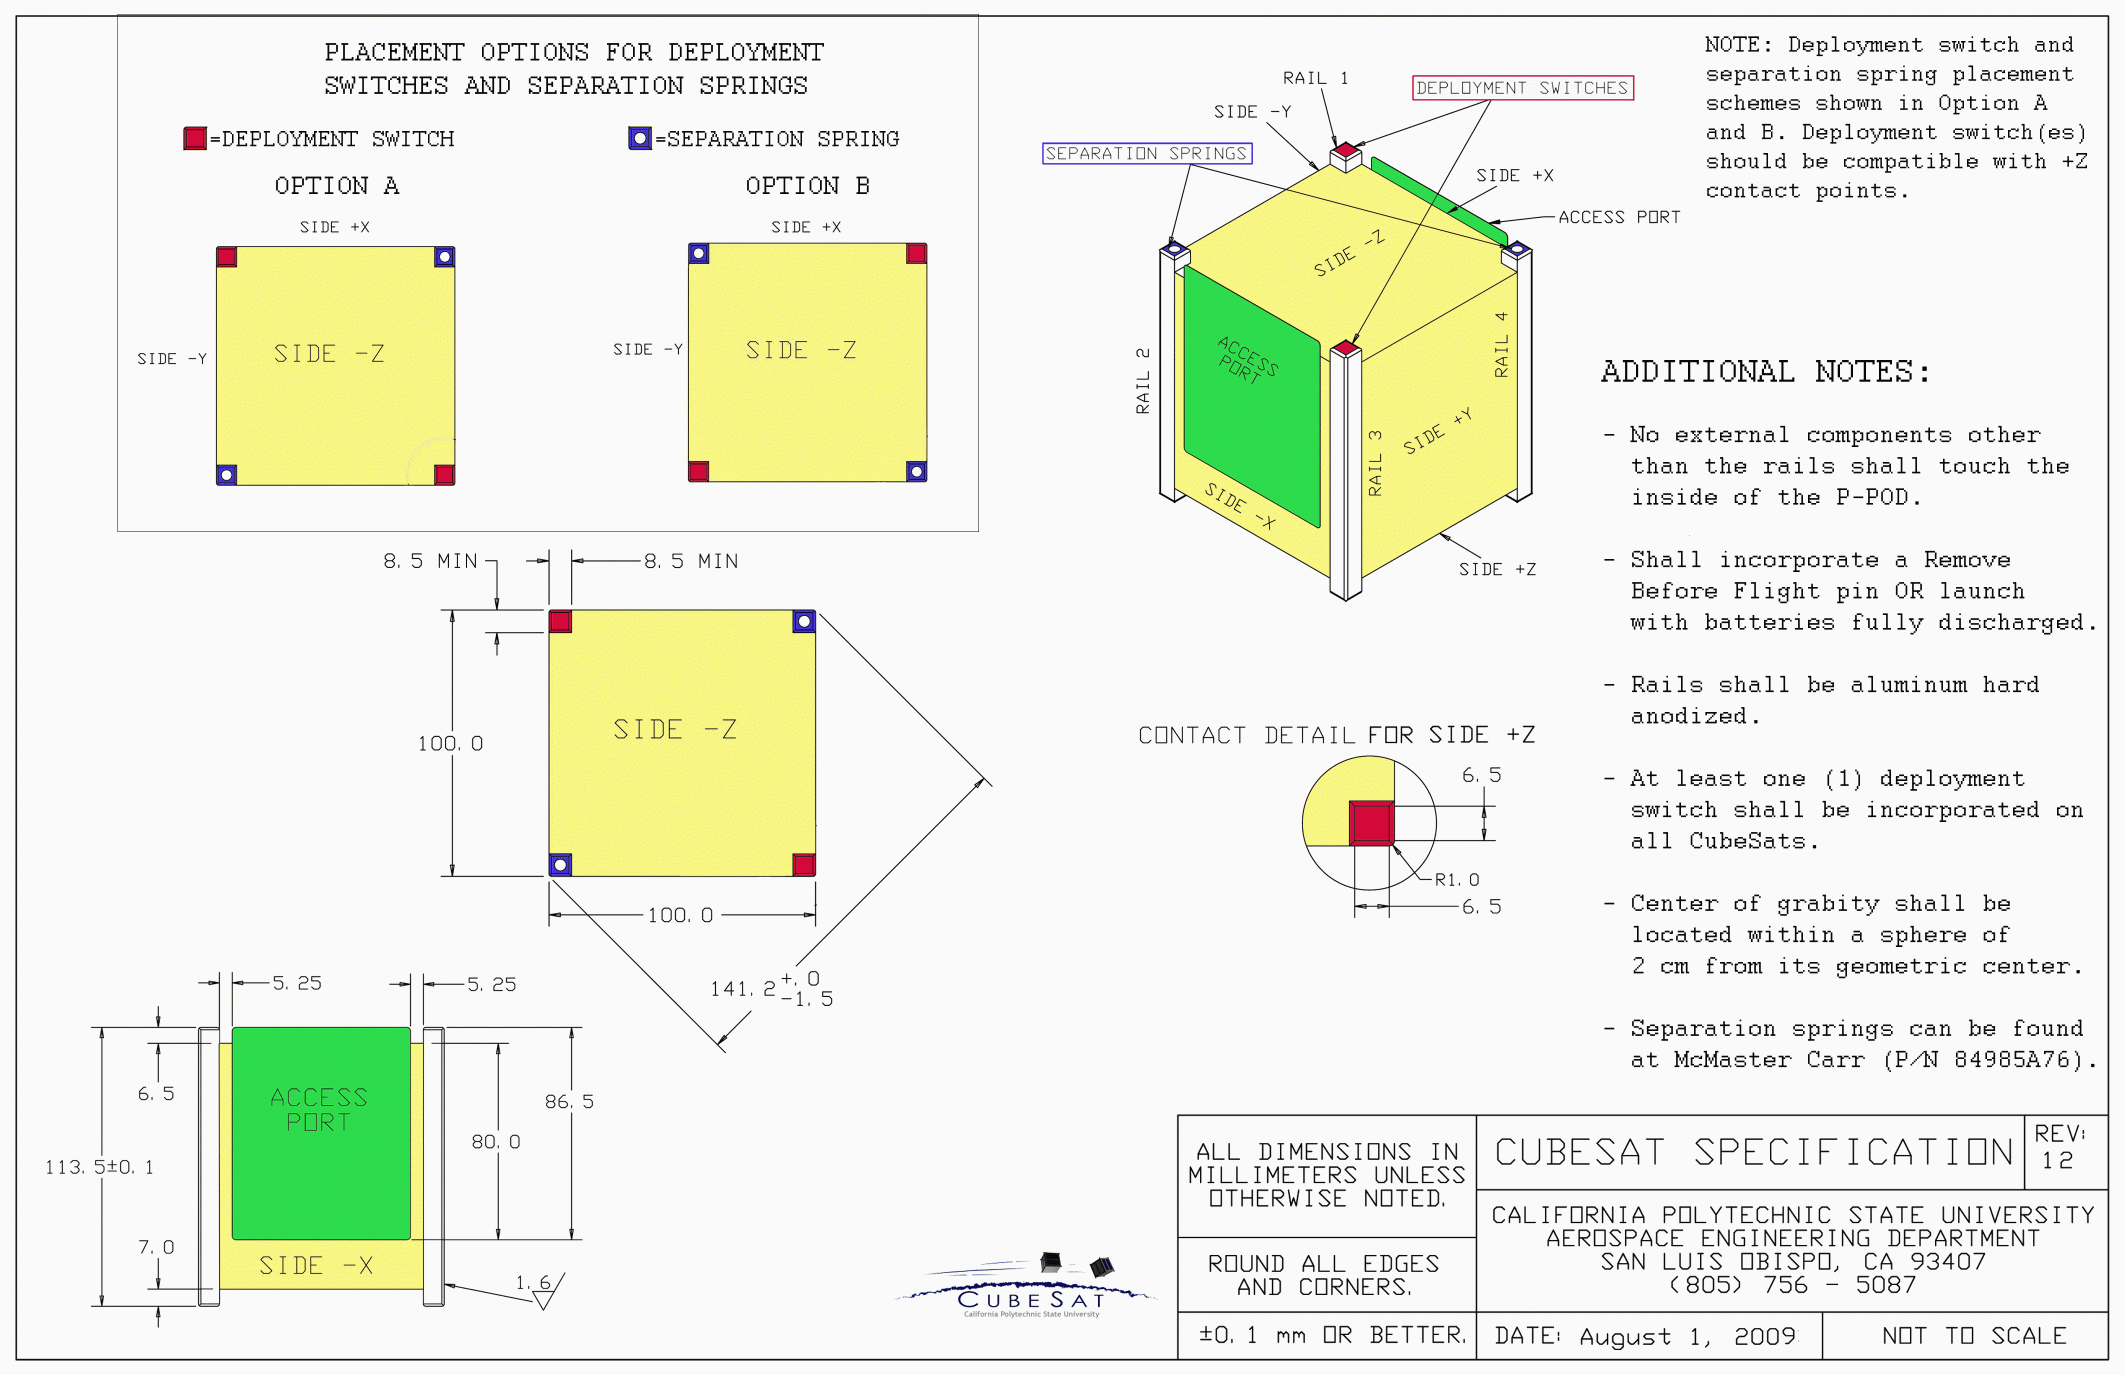
\includegraphics[scale=0.6]{./sections/SatelliteDesign/images/CubeSatDesign}
\centering
\caption{Dimensions of a 1U CubeSat \cite{cubesatdimensions}}
\end{figure}

\subsubsection{Structure}

\paragraph{}The mission of the structure is to sustain and protect all the electronic devices carried by the satellite in order to fulfill the mission requirements. In order to ensure that all the electronic and mechanic systems can be mounted upon the structure, a high compatibility between these systems is required.

The structure used will be provided by Innovative Solutions In Space (ISIS). Among its features it is worth mentioning that it can withstand the high range of temperature it will face in the space (-40ºC to 80ºC) and it is highly compatible with almost every physical system that will be used. Additionally, it is a low mass structure (304.3g) and it can support different configurations within it.

\paragraph{}Since the configuration within the CubeSat will not be as common as other configuration options within of current operational CubeSats because the mission of the project is to relay fast and reliable communication with the ground station and the other satellites, it is a really important point that the structure is highly flexible regarding the arrangement of the subsystems that it will carry.

\subsubsection{Deployments}

\paragraph{}\textbf{FALTA}


\subsubsection{Thermal protection}
\paragraph{}The thermal protection system protect the CubeSat from thermal shocks. The satellite must remain in a optimal range of temperatures,despite the external temperature. It consists of various insulating materials and thermal conductors in order to maintain it within acceptable temperatures.

\paragraph{} 
Thermal protection system is needed to mantain the temperature of the CubeSat inside the range operational temperatures of the differents subsystems. In space, the CubeSat can suffer extreme temperatures, both below zero and above zero, and thermal protection must guarantee the correct operation of all devices. Furthermore, thermal protection remove heat caused by other systems.

\paragraph{} 
Currently, the element most used as thermal protection in the aerospace industry is multilayer insulation (MLI). The MLI comply requirements previously explained and consists of multiple thin layers. The main objective of the MLI is to reduce the heat by radiation because the heat by convection or conduction don't affect so much.

\paragraph{} 
After a market study, Dunmore Aerospace company has been chosen to provide us its MLI product. Specially, the product is the Dunmore Aerospace Satkit and it is made for small satellites for low earth orbit.

\subsubsection{Study of the commercial available options}

\begin{longtable}{| l | r | r | }
\hline
\rowcolor[gray]{0.80}	\textbf{System} &  \textbf{Brand and model}     & \textbf{Price per unit (\euro)}   \\
\hline
\endfirsthead

	   ~3U Structure & ISIS & 3900) \\
	   ~Thermal Protection 1 & EMPTY & EMPTY \\
	\hline

\caption{Options studied}
\label{epsoptionstable}
\end{longtable}
